%% PNAStwoS.tex
%% Sample file to use for PNAS articles prepared in LaTeX
%% For two column PNAS articles
%% Version: Apr 15, 2008 
 

%% BASIC CLASS FILE
\documentclass{pnastwo}

%% ADDITIONAL OPTIONAL STYLE FILES
\usepackage[dvips]{graphicx}
\usepackage{PNAStwoF}
\usepackage{amssymb,amsfonts,amsmath}
\usepackage{url}

%% OPTIONAL MACRO DEFINITIONS
\def\s{\sigma}



\usepackage{url}
%\usepackage{graphics}

\begin{document}

\title{SI: Tackling soil diversity with the assembly of large, complex metagenomes }

\author{Adina Chuang Howe\affil{1}{Microbiology and Molecular Genetics, Michigan State
University, East Lansing, MI, USA}\affil{2}{Plant, Soil, and Microbial Sciences,
Michigan State University, East Lansing, MI, USA}, 
Janet Jansson\affil{3}{Department of Energy
(DOE) Joint Genome Institute, Walnut Creek, CA, USA}\affil{4}{Lawrence Berkeley
National Laboratory, Earth Sciences Division, Berkeley, CA, USA}, 
Stephanie A. Malfatti\affil{3}{},
Susannah G. Tringe\affil{3}{}, 
James M. Tiedje\affil{1}{}\affil{2}{}, and 
C. Titus Brown\affil{1}{}\affil{5}{Computer Science and Engineering, Michigan State University}}

\contributor{Submitted to Proceedings of the National Academy of Sciences
of the United States of America}
\maketitle

\begin{article}
\section*{Supplementary Methods}
\subsection*{Assembly Methods.} The HMP mock community dataset and its available draft reference
genomes were used to evaluate our approaches towards data reduction
and partitioning for \emph{de novo} metagenomic assembly.  Reads of
the mock community dataset were initially digitally normalized to a
coverage threshold of 20 (as previously described in \cite{browndiginorm}),
reducing the total number of reads from 14 to 11 million.
Additionally, to remove possible sequencing artifacts associated with
high coverage sequences (previously described in Howe et al., in preparation),
highly-abundant sequences (20-mers present at coverage greater than
50-fold) were filtered and the dataset was further normalized to a
coverage of 10, resulting in a total of 9 million reads (Fig.
3).  Finally, the remaining reads were divided into
disconnected sets of reads resulting in a total of 85,818 partitions
containing greater than five reads (summarized in
Table 1).  The entire assembly pipeline for the mock community is described in
detail in an IPython notebook available for download at 
\url{http://nbviewer.ipython.org/urls/raw.github.com/ngs-docs/ngs-notebooks/
master/ngs-70-hmp-diginorm.ipynb}
and 
\url{http://nbviewer.ipython.org/urls/raw.github.com/ngs-docs/ngs-notebooks/
master/ngs-71-hmp-diginorm.ipynb}. 

\subsection*{Datasets.}
In this study, we examined two large soil metagenomes generated from
soils collected from Iowa corn and native prairie soils.  Sequencing
was performed at the DOE Joint Genome Institute (Walnut Creek, CA).  Soil metagenomes included both
GAII and HiSeq Illumina paired-end libraries (76x2 and 114x2).  
Reads were quality trimmed at basepair locations where Phred scores indicated a score of
'2'.  The total quality-trimmed reads in the Iowa corn and prairie
datasets were 1.8 million and 3.3 million, respectively.  Quality-trimmed unassembled reads used for Iowa corn and prairie assemblies are available on the MG-RAST metagenomics analysis server, in project IDs 6368 (metagenomes 
4539514.3, 
4539515.3, 
4539516.3, 
4539517.3, 
4539518.3, 
4539519.3, 
4539520.3, 
4539521.3, 
4539522.3, 
4539523.3, 
4539524.3, 
4539525.3, 
4539526.3, 
4539527.3, and
4539528.3) 
and 6377 (metagenomes  4539571.3, 
4539572.3, 
4539573.3, 
4539574.3, 
4539575.3, 
4539576.3, 
4539577.3, 
4539578.3, 
4539579.3, 
4539580.3, 
4539581.3, 
4539582.3, 
4539583.3, 
4539584.3, 
4539585.3, 
4539586.3, 
4539587.3, 
4539588.3, 
4539589.3, 
4539590.3, 
4539591.3, 
4539592.3, 
4539593.3, and
4539594.3), respectively.  The direct urls for these metagenome collections are as follows for the Iowa corn and prairie unassembled reads:  \url{http://metagenomics.anl.gov/linkin.cgi?project=6368} and \url{http://metagenomics.anl.gov/linkin.cgi?project=6377}.
We also
include a human gut mock community dataset (combined from SRA
SRX055381 and SRX055380).  For this mock community dataset, DNA from
bacterial isolates originally recovered from within or on the human
body was mixed together at staggered concentrations (over 5 orders of
magnitude based on genomic DNA concentrations) and sequenced.  The
mock community dataset originally contained 14.5 million reads.

To evaluate our approach, we added simulated reads from either a
single \emph{E. coli} (str. K-12 substr DH10B) or five \emph{E. coli} strains (K-12
substr DH10B, E24377, O147:H7 str. EC4115, UMN026, SE15) into select
metagenomes.  We computationally generated 100 bp reads from each
reference genome to a coverage of 10x and with a 2\% error rate and
subsequently randomly shuffled these reads.

\subsection*{Estimation of assembly requirements for soil metagenomes.}
Subsets of the Iowa corn metagenome were assembled with the Velvet
assembler (v1.2.07) with the following parameters: velveth K=45,
-short and velvetg -exp\_cov auto -cov\_cutoff auto, -scaffolding no.
The time and memory for each assembly was estimated up to a maximum of
150 hours and 100 GB.

\subsection*{Digital normalization.}
In order to reduce the dataset size, extraneous sequences for which sufficient coverage were available for assembly  were removed through digital normalization.  Digital normalization is further described in \cite{browndiginorm}.  
For the mock community dataset, digital normalization was performed with the
following parameters: K=20, coverage=20, and Bloom filter size = 1 GB
x 4.  For Iowa corn metagenome, digital normalization parameters were
as follows: K=20, coverage=20, and Bloom filter size = 48 GB x 4.
Similar parameters were used for the Iowa prairie metagenome, with the
exception that the Bloom filter size was 60 GB x 4.

\subsection*{Removal of high abundance sequences.}
To eliminate known sequencing artifacts in Illumina metagenomes, high abundance 
sequences (coverage
greater than 50) were removed using the count-min-sketch datastructure
used for digital normalization.  For the relatively high coverage mock
community dataset, filtered reads were subsequently normalized to a
coverage of 10 (K=20, bloom filter size = 1 GB x 4).

\subsection*{Partitioning and assembly of disconnected reads.}
The partitioning approach divides a larger dataset into groups of reads which share overlaps, dividing the dataset into subsets of connectivity.  Disconnected partitions of the assembly de Bruijn graph (assembly) graph were separated by loading normalized filtered datasets into a probabilistic
representation of the assembly graph as described in \cite{Pell:2012cq}.
Partitions containing less than five reads were discarded.  Each
partition was subsequently assembled using the Velvet assembler with
the same setting as described above, with the exception that K=35-59
and shortPaired setting was used for paired end reads.  The resulting
contigs greater than 300 bp from multiple-K assemblies were
dereplicated with CD-HIT (\cite{Fu:2012jk}, 99\% similarity) and merged with
Minimus2 \cite{Sommer:2007p1253}.   Additionally, partitons were also assembled with 
Meta-IDBA \cite{Peng:2011p898} and SOAPdenovo \cite{Li:2010jz}).  Meta-IDBA assembly parameters were as follows:  idba --mink 25 --maxk 50 --minCount 0.  SOAPdenovo assembly parameters were as follows:  SOAPdenovo-31mer all -K 31 -p 8, asm\_flags=1, and single and paired reads were separated and used for assembly.

\subsection*{Comparing coverage of reference genomes by reads.}
Reads in the HMP mock unfiltered and filtered datasets were mapped
back to originating genomes using default settings in Bowtie2
\cite{bowtie}.  For cases where reads could be mapped back to multiple
genomes, a single genome was randomly selected to be identified with
each read.  Sequencing coverage was estimated for the whole genome as
the median base pair coverage for all base pairs in the reference
genome.

\subsection*{Read coverage by assemblies.}
All quality trimmed reads for Iowa corn and prairie were aligned with
assembled contigs (length greater than 300 bp) using default
parameters in Bowtie2 \cite{bowtie}.  Paired end reads were evaluated according to
concordance with paired end library preparation (i.e. paired end reads
on opposite DNA strands) and the alignment of both pairs of reads to
an assembled contig.  The base pair coverage of each contig was
estimated with the median base pair coverage of all reads across the
length of the contig.  Additionally, for each position in a contig
(with the exception of the external 100 bp on each end), the
percentage of the mapped consensus base pairs was calculated.  The
fraction of positions with greater than 95\% base consensus was
calculated to estimate the presence of polymorphisms within the
assembled contig.  

Read coverage was also used to compare sequences without known annotations between the corn and prairie soil metagenomes.  Contigs shared with another metagenome were characterized by 
having a minimum total of 10 bp median coverage among all available samples as well as present in all samples.  All identified shared contigs were also dereplicated with CD-HIT (99\% similarity) and the best representative chosen.

\subsection*{Annotation of assemblies.}
Assembled contigs and their corresponding median bp coverage for the
Iowa corn and prairie metagenomes were upload into MG-RAST annotation
pipeline \cite{Meyer:2008db} and are available on MG-RAST as 4504979.3 (Iowa corn)
and 4504798.3 (Iowa Prairie).  The resulting MG-RAST blat annotations
were compared to the M5NR database using a maximum e-value of 1e-5, a
minimum identity of 60\%, and a minimum alignment length of 15 aa unless otherwise noted.
The annotated metagenome for Iowa corn can be found at
\url{http://metagenomics.anl.gov/linkin.cgi?metagenome=4504797.3} and 
Iowa prairie at \url{http://metagenomics.anl.gov/linkin.cgi?metagenome=4504798.3}.
MG-RAST KEGG KO ids were placed on metabolic pathways available through  
 \url{http://www.genome.jp/kegg/tool/map_pathway2.html}.

\subsection*{Comparing assemblies.}
Resulting assemblies (contigs greater than 300 bp) were compared using
the total number of contigs, assembly length, and maximum contig size
for each assembly.  Assemblies were also aligned to each other using
blastn and the resulting coverage of each assembly was calculated.  In
the case of the mock community, the resulting assemblies were also
aligned to sequenced draft genomes of the original isolates and, if
applicable, spiked reference genomes. Abundance of assembled contigs
and reference genomes were estimated by mapping raw reads with Bowtie
(allowing up to 2 mismatches for a match).  The median base pair
coverage was used to estimate abundances.  Associated assembled
contigs (greater than 300 bp) from the unfiltered and filtered
(digital normalized) assemblies were identified using a blastn
alignment (requiring E-value cutoff of 1e-5).  Contigs were associated
with reference genomes through an identical alignment approach.

\subsection*{Statistical comparison of assemblies.}
The reference-based abundance (from reads mapped to reference genomes)
and assembly-based abundance (from reads mapped to contigs) of genomes
were compared.  Using a one-directional, paired t-test of squared
deviations, the abundance estimates of the unfiltered and filtered
assemblies were compared.  The mean and standard deviation of 
the abundances of unfiltered contigs, filtered contigs, and reference genes
were 6.8 +/- 7.1, 8.1 +/- 7.7, and 7.8 +/- 5.2, respectively.  We expected the 
filtered assembly to have increased accuracy due to a reduction of errors (e.g. normalization
and high abundance filtering) and used a one-sided t-test which
indicated that abundance estimations from the filtered assembly were
significantly closer to predicted abundances from reference genomes
(n=28,652, p-value of 0.032).


\begin{thebibliography}{1}

\bibitem{browndiginorm}
Brown, C.~T, Howe, A, Zhang, Q, Pyrkosz, A.~B,  \& Brom, T.~H.
\newblock (2012) A reference-free algorithm for computational normalization of
  shotgun sequencing data.
\newblock {\em arXiv:1203.4802}.

\bibitem{Pell:2012cq}
Pell, J, Hintze, A, Canino-Koning, R, Howe, A, Tiedje, J.~M,  \& Brown, C.~T.
\newblock (2012) {Scaling metagenome sequence assembly with probabilistic de
  Bruijn graphs}.
\newblock {\em Proceedings of the National Academy of Sciences of the United
  States of America} {\bf 109}, 13272--13277.

\bibitem{Fu:2012jk}
Fu, L, Niu, B, Zhu, Z, Wu, S,  \& Li, W.
\newblock (2012) {CD-HIT: accelerated for clustering the next generation
  sequencing data.}
\newblock {\em Bioinformatics (Oxford, England)}.

\bibitem{Sommer:2007p1253}
Sommer, D.~D, Delcher, A.~L, Salzberg, S.~L,  \& Pop, M.
\newblock (2007) Minimus: a fast, lightweight genome assembler.
\newblock {\em Bmc Bioinformatics} {\bf 8}, 64.

\bibitem{bowtie}
Langmead, B \& Salzberg, S.
\newblock (2012) Fast gapped-read alignment with bowtie 2.
\newblock {\em Nature Methods} {\bf 9}, 357--359.

\bibitem{Meyer:2008db}
Meyer, F, Paarmann, D, D'Souza, M, Olson, R, Glass, E.~M, Kubal, M, Paczian, T,
  Rodriguez, A, Stevens, R, Wilke, A, Wilkening, J,  \& Edwards, R.~A.
\newblock (2008) {The metagenomics RAST server - a public resource for the
  automatic phylogenetic and functional analysis of metagenomes.}
\newblock {\em BMC bioinformatics} {\bf 9}, 386.

\bibitem{Peng:2011p898} Peng, Y, Leung, H. C.~M, Yiu, S.~M, \& Chin, F. Y.~L.
\newblock (2011) Meta-idba: a de novo assembler for metagenomic data. \newblock
{\em Bioinformatics} {\bf 27}, i94--101.



\bibitem{Li:2010jz} Li, R, \& et al. \newblock
(2010) {De novo assembly of human genomes with massively parallel short read
sequencing}. \newblock {\em Genome Research} {\bf 20}, 265--272.
\end{thebibliography}
\end{article}

\renewcommand{\thepage}{S\arabic{page}}  
\renewcommand{\thesection}{S\arabic{section}}   
\renewcommand{\thetable}{S\arabic{table}}   
\renewcommand{\thefigure}{S\arabic{figure}}
\


\begin{figure}
\center{\includegraphics[width=.7\textwidth]{./figures/reference_coverage.eps}}
\caption{Coverage of reference genomes (estimated actual coverage shown in parentheses) by sequences in unfiltered and normalized filtered unassembled reads and assembled contigs.}
\label{coverage1}
\end{figure}


\begin{figure}
\centerline{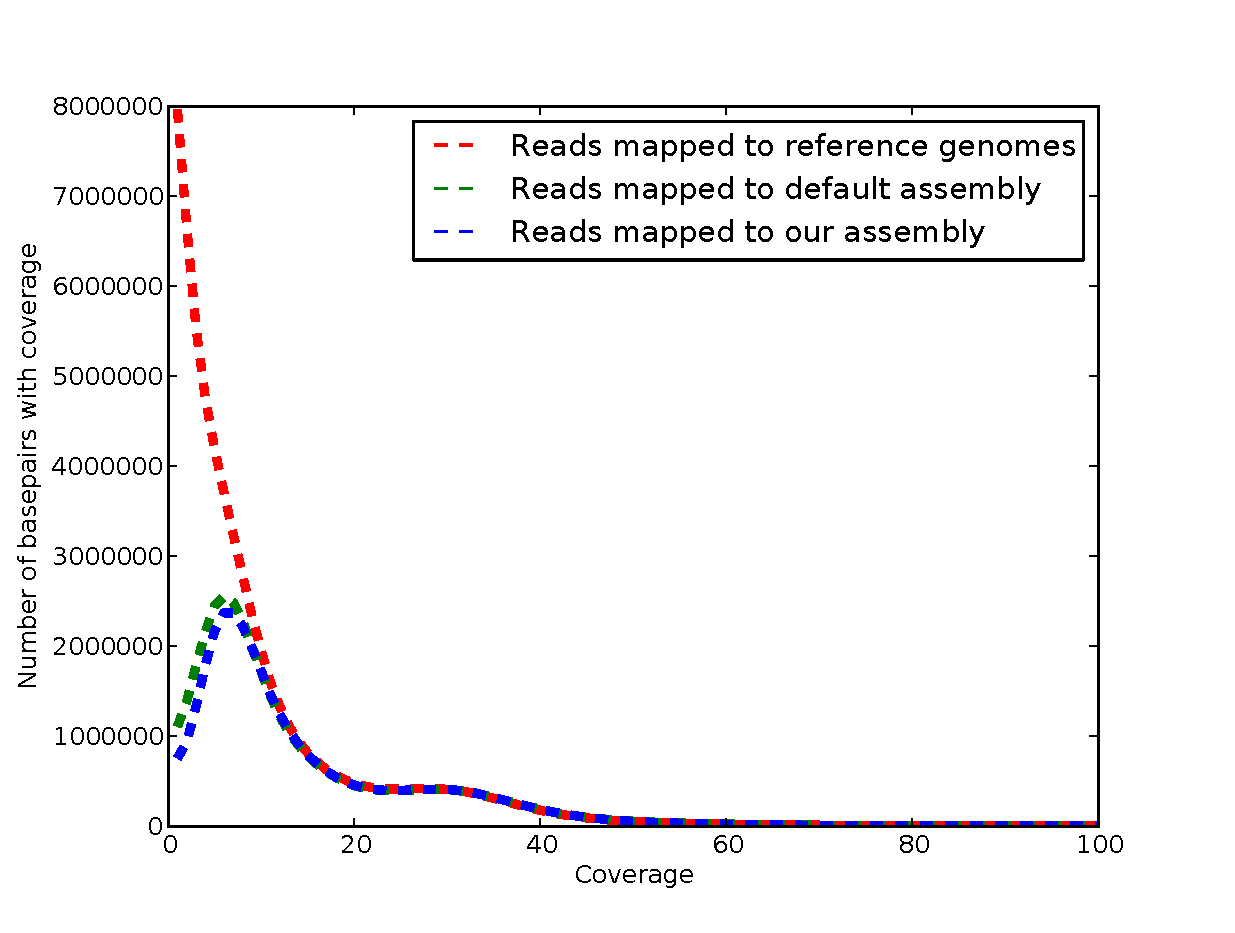
\includegraphics[width=.7\textwidth]{./figures/coverage.eps}}
\caption{For the HGMC datatset, the number of basepairs with specified coverage for reads which
  map to reference genomes and unfiltered and filtered assembled
  contigs greater than 300 bp.}
\label{coveragehmp}
\end{figure}






\begin{figure}
\begin{center}
\centerline{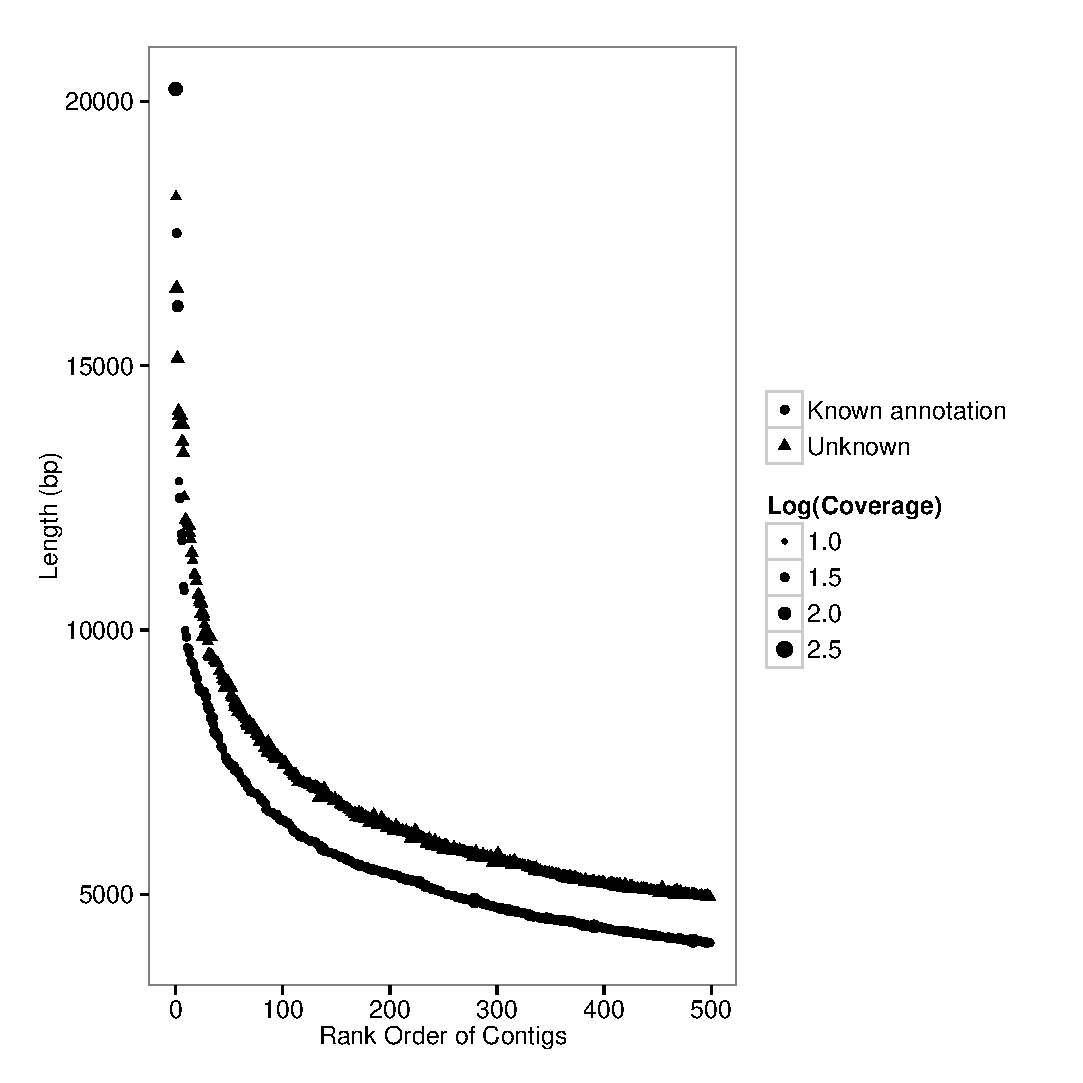
\includegraphics[width=.7\textwidth]{./figures/corn-cov-len-500.eps}}
\caption{Length distribution of longest assembled corn metagenome contigs with and without similarity to known sequences.  Unknown contigs were defined as sequences with no annotated gene regions.  Coverage (log-scale) of these sequences is also shown by the size of marker. }
\label{cornlength}
\end{center}
\end{figure}

\begin{figure}
\begin{center}
\centerline{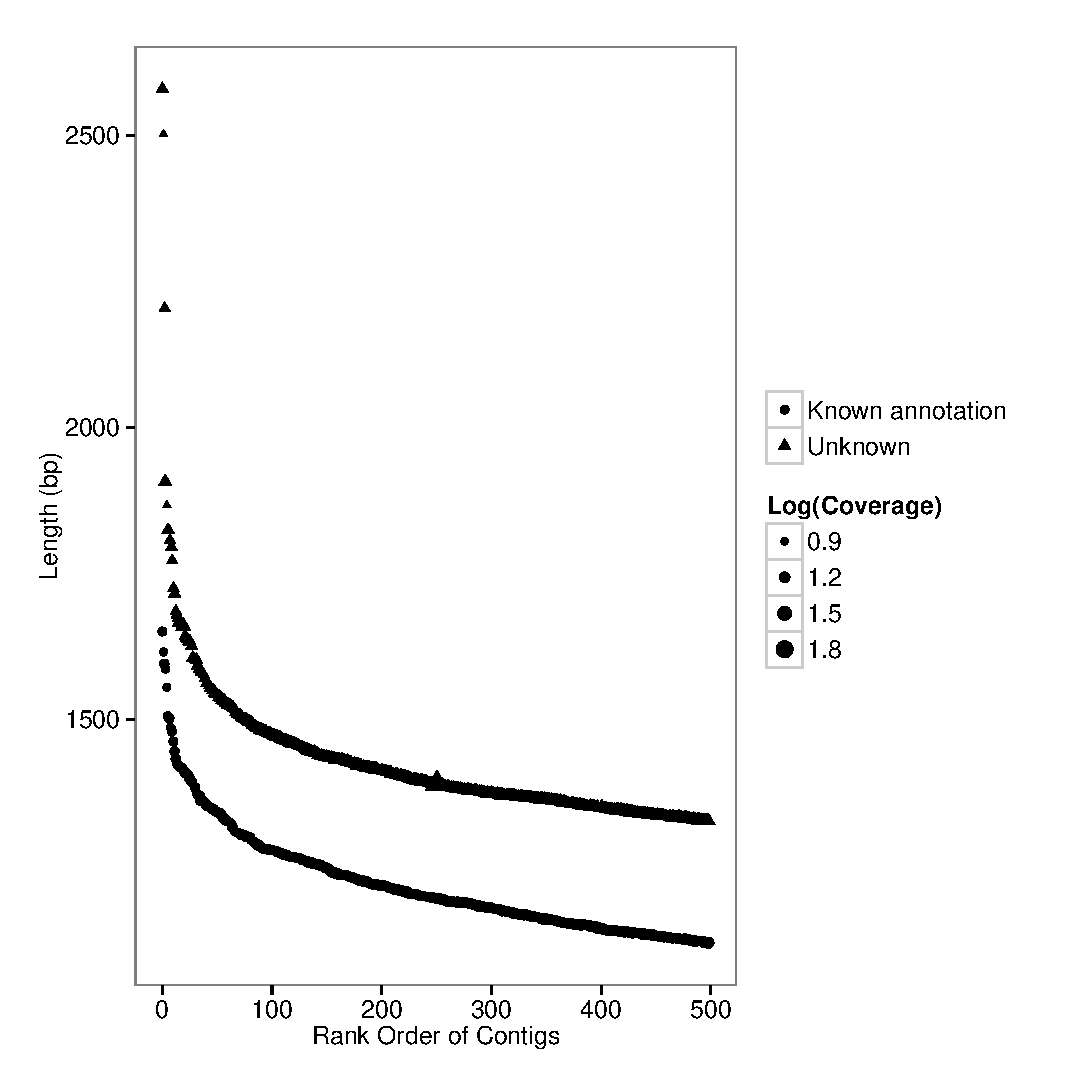
\includegraphics[width=.7\textwidth]{./figures/prairie-cov-len-500.eps}}
\caption{Length distribution of longest assembled prairie metagenome sequences with and without similarity to known sequences.  Coverage (log-scale) of these sequences is also shown by the size of marker. }
\label{prairielength}
\end{center}
\end{figure}


\begin{figure}
\begin{center}
\centerline{\includegraphics[width=.7\textwidth]{./figures/read-len.eps}}
\caption{Distribution of alignment lengths of unassembled corn metagenomes (red) and assembled corn metagenome (blue) to sequences in KEGG KO database for alignments meeting the following criteria:  E-value less than 1e-10, identity > 60\%, alignment length > 30 aa.  Average alignment lengths for unassembled and assembled sequences were 88 and 32 aa, respectively.   Total number of unique  KEGG KO proteins identified in unassembled and assembled datasets vary depending on blat criteria as shown for varying alignment lengths.}
\label{length-aln}
\end{center}
\end{figure}


\begin{figure}
\begin{center}
\centerline{\includegraphics[width=.7\textwidth]{./figures/metabolism_kegg_pathway_all.eps}}
\caption{KEGG pathways sharing similarity with assembled soil metagenome sequences (black=combined corn and prairie, blue = prairie only, red = corn only.}
\label{kegg}
\end{center}
\end{figure}



\begin{table}
\caption{HMGC dataset reference genomes estimated sequencing depth
  (median bp coverage of reads), number of partitions, total length
  (bp), coverage of reference genomes by unfiltered reads (UF Cov),
  coverage of reference genomes by normalized filtered reads (F Cov), coverage of
  reference genomes by unfiltered assembled contigs (UFA Cov), and
  coverage of reference genomes by normalized filtered assembled contigs (FA
  Cov).}
\begin{tabular}{@{\extracolsep{\fill}}l c c c c c c c}
\hline Reference Genome & Coverage & No. Partitions & Length (bp) & UF
Cov (bp) & F Cov (bp) & UFA Cov & FA Cov \\ \hline
NC\_005008.1 &
2,412 & 9 & 4,439 & 4,439 & 1,058 & 100 \% & 28 \% \\
NC\_005007.1 &
549 & 16 & 4,679 & 4,679 & 4,585 & 100 \% & 77 \% \\
NC\_005003.1 &
533 & 21 & 6,585 & 6,585 & 6,441 & 100 \% & 64 \% \\
NC\_005006.1 &
253 & 2 & 8,007 & 8,004 & 7,953 & 100 \% & 100 \% \\
NC\_005004.1 &
112 & 52 & 24,365 & 24,358 & 24,291 & 100 \% & 83 \% \\
NC\_009084.1 &
85 & 3 & 11,302 & 11,295 & 11,270 & 100 \% & 100 \% \\
NC\_005005.1 & 74
& 12 & 17,261 & 17,202 & 17,180 & 100 \% & 100 \% \\
NC\_000958.1 & 71
& 73 & 177,466 & 177,261 & 174,614 & 100 \% & 95 \% \\
NC\_000959.1 & 52
& 37 & 45,704 & 44,974 & 43,557 & 100 \% & 92 \% \\
NC\_009083.1 &
48 & 2 & 13,408 & 13,405 & 13,383 & 100 \% & 100 \% \\
NC\_001264.1 & 40
& 63 & 412,348 & 410,970 & 403,553 & 100 \% & 99 \% \\
NC\_001263.1 & 32
& 546 & 2,648,638 & 2,634,512 & 2,589,566 & 100 \% & 99 \% \\
NC\_004461.1 & 30
& 476 & 2,499,279 & 2,498,081 & 2,492,248 & 100 \% & 98 \% \\
NC\_009008.1 &
29 & 14 & 37,100 & 36,585 & 33,250 & 94 \% & 96 \% \\
NC\_010079.1 &
29 & 442 & 2,872,915 & 2,298,758 & 2,157,196 & 100 \% & 92 \% \\
NC\_007490.1 & 27
& 27 & 100,828 & 99,385 & 93,550 & 100 \% & 96 \% \\
NC\_009007.1 &
24 & 92 & 114,045 & 108,526 & 97,860 & 100 \% & 96 \% \\
NC\_007489.1 & 18
& 12 & 105,284 & 102,212 & 96,169 & 100 \% & 99 \% \\
NC\_004350.1 & 16
& 131 & 2,030,921 & 2,029,376 & 2,025,544 & 100 \% & 99 \% \\
NC\_007488.1 & 13
& 30 & 114,178 & 103,351 & 93,637 & 100 \% & 99 \% \\
NC\_007493.1 & 13
& 628 & 3,188,609 & 2,919,441 & 2,681,855 & 100 \% & 99 \% \\
NC\_007494.1 & 13
& 262 & 943,016 & 862,781 & 788,626 & 100 \% & 98 \% \\
NC\_009085.1 &
11 & 683 & 3,976,747 & 3,939,190 & 3,936,208 & 99 \% & 99 \% \\
NC\_009515.1 & 9
& 552 & 1,853,160 & 1,828,231 & 1,826,639 & 99 \% & 98 \% \\
NC\_009614.1 & 7
& 7,751 & 5,163,189 & 4,899,622 & 4,896,808 & 81 \% & 82 \% \\
NC\_000915.1 & 6
& 2,888 & 1,667,867 & 1,581,502 & 1,581,024 & 78 \% & 79 \% \\
NC\_003028.3 & 6
& 4,123 & 2,160,842 & 2,047,832 & 2,037,347 & 78 \% & 78 \% \\
NC\_000913.2 & 6
& 5,913 & 4,639,675 & 4,080,605 & 4,074,119 & 84 \% & 85 \% \\
NC\_006085.1 & 6
& 6,459 & 2,560,265 & 2,169,547 & 2,169,056 & 59 \% & 64 \% \\
NC\_003112.2 & 4
& 9,269 & 2,272,360 & 1,655,023 & 1,626,301 & 28 \% & 33 \% \\
\hline
\end{tabular}
\label{ref-summary}
\end{table}


\begin{table}
\caption{Assembly comparisons of HMGC unfiltered (UF) and normalized filtered (NF) or
  filtered/partitioned (FP) HMGC datasets using different
  assemblers (Velvet (V), Meta-IDBA (M) and SOAPdenovo (S)).  Assembly
  content similarity is based on the fraction of alignment of
  assemblies and similarly, the coverage of reference genomes is based
  on the alignment of assembled contigs to reference genomes (RG).}
\begin{tabular}{@{\extracolsep{\fill}}lcccc}
Assembly Comparison & Percent Similarity & RG Coverage & Assembler \\
\hline
UF vs. NF & 95\% & 43.3\% / 44.5\% & V \\
UF vs. FP & 95\% & 43.3\% / 44.4\% & V\\
UF vs. FP & 93\% & 46.5\% / 45.4\% & M\\ 
UF vs. FP & 98\% &  46.2\% / 46.4\% & S\\
\hline
\end{tabular}
\label{assembly-compare}
\end{table}

\begin{table}
\caption{Longest contigs in the corn and prairie soil metagenome with similarity to the RefSeq database. (*Indicates SEED database origin if no RefSeq organismal annotation available.)}
\begin{tabular}{@{\extracolsep{\fill}}lccl}
Contig ID & Length (bp) & Coverage &  Function \& Organsim \\
 \hline
iowa-corn-3-pass.4582796.20234*	&	20234	&	138	&	Probable poly(beta-D-mannuronate) O-acetylase (EC 2.3.1.-)	\\
	&		&		&	Cyanothece sp PCC 7425	\\
iowa-corn-3-pass.4606542.17507	&	17507	&	30	&	hypothetical protein	\\
	&		&		&	Pseudomonas phage PaP2	\\
iowa-corn-3-pass.4578484.16126	&	16126	&	62	&	hypothetical protein	\\
	&		&		&	Pseudomonas phage PaP2	\\
iowa-corn-3-pass.4583611.12814	&	12814	&	18	&	replication factor C large subunit	\\
	&		&		&	Candidatus Methanoregula boonei 6A8	\\
iowa-corn-3-pass.4594771.12496	&	12496	&	35	&	carbonic anhydrase	\\
	&		&		&	Psychromonas ingrahamii 37	\\
iowa-corn-3-pass.4596152.11816	&	11816	&	25	&	ribonuclease Z	\\
	&		&		&	Thermococcus kodakarensis KOD1	\\
iowa-corn-3-pass.4616349.11691	&	11691	&	25	&	precorrin-3B C17-methyltransferase	\\
	&		&		&	Nitrosopumilus maritimus SCM1	\\
iowa-corn-3-pass.4592007.10823	&	10823	&	22	&	hydroxymethylglutaryl-CoA reductase, degradative	\\
	&		&		&	Staphylothermus marinus F1	\\
iowa-corn-3-pass.4589906.10747	&	10747	&	23	&	RdgB/HAM1 family non-canonical purine NTP pyrophosphatase	\\
	&		&		&	Roseiflexus castenholzii DSM 13941	\\
iowa-corn-3-pass.4559414.9998&	9998	&	19	&	heparan N-sulfatase	\\
	&		&		&	Blastopirellula marina DSM 3645	\\
iowa-prairie-3-pass.6326293.1650	&	1650	&	11	&	PAS/PAC sensor signal transduction histidine kinase	\\
	&		&		&	Marinobacter aquaeolei VT8	\\
iowa-prairie-3-pass.6215171.1615*	&	1615	&	9	&	Beta-mannosidase (EC 3.2.1.25)	\\
	&		&		&	Acidobacteria bacterium Ellin345	\\
iowa-prairie-3-pass.6327344.1595	&	1595	&	12	&	glycosyl transferase, group 2 family protein	\\
	&		&		&	Bacillus cereus ATCC 10987	\\
iowa-prairie-3-pass.6326016.1586	&	1586	&	10	&	hypothetical protein	\\
	&		&		&	Dechloromonas aromatica RCB	\\
iowa-prairie-3-pass.6155396.1555	&	1555	&	9	&	peptidase S33, proline iminopeptidase 1	\\
	&		&		&	Pseudomonas syringae pv. syringae B728a	\\
iowa-prairie-3-pass.6285889.1505	&	1505	&	11	&	AMP-dependent synthetase and ligase	\\
	&		&		&	Chloroflexus sp. Y-400-fl	\\
iowa-prairie-3-pass.6293899.1502	&	1502	&	13	&	beta-lactamase	\\
	&		&		&	Flavobacterium johnsoniae UW101	\\
iowa-prairie-3-pass.5906709.1488	&	1488	&	7	&	peptidase M24	\\
	&		&		&	Chitinophaga pinensis DSM 2588	\\
iowa-prairie-3-pass.6216765.1484	&	1484	&	10	&	amine oxidase	\\
	&		&		&	Candidatus Solibacter usitatus Ellin6076	\\
iowa-prairie-3-pass.6224149.1479	&	1479	&	12	&	phosphoribosylglycinamide formyltransferase 	\\
& & & Bacteroides sp. 2\_1\_16\\
\hline
\end{tabular}
\label{mgrast}
\end{table}


\end{document}

